\chapter{Operads and their algebras} \label{actionoperad} 

Before we can talk about the main focus of this paper, the free $\mathrm{E}G$-algebras on $n$ invertible objects, we will need to work our way through several intermediate concepts. This chapter will cover the background material needed to understand each of these other structures in turn --- monoidal categories, operads, action operads, $G$-operads, and operad algebras. Most of this content is due to other authors, and the reader is encouraged to refer to the given sources if they are interested in a more complete analysis of any of the featured topics. 

\section{Basic definitions}

In this section we shall briefly review some standard definitions from category theory that will be used throughout the paper. Everything in this section can be found in any good introductory text on category theory, such as the foundational `Categories for the Working Mathematician' \cite{cwm} by Saunders Mac Lane.

We will start with the notion of an adjunction.

\begin{defn} Let $C$ and $D$ be categories, and $F: C \to D$, $G: D \to C$ be functors. Then we say that $F$ is \emph{left adjoint} to $G$, and that $G$ is \emph{right adjoint} to $F$, if for any objects $X$ in $C$ and $Y$ in $D$ there exists an isomorphism
\begin{eq*} D\big( \, F(X), \,  Y \, \big) \quad \cong \quad C\big( \, X, \, G(Y) \, \big) \end{eq*}
natural in both variables. Equivalently, $F$ and $G$ are adjoints if there exist natural transformations $\eta: \mathrm{id}_{C} \Rightarrow G \circ F$ and $\epsilon : F \circ G \Rightarrow \mathrm{id}_{D}$ which obey the so-called zig-zag identities,
\begin{eq*} \begin{tikzcd}
F \ar[rr, "\mathrm{id}_F \circ \eta"] \ar[ddrr, "\mathrm{id}_F"'] & & FGF \ar[dd, "\epsilon \circ \mathrm{id}_F"] & \quad & G \ar[rr, "\eta \circ \mathrm{id}_G"] \ar[ddrr, "\mathrm{id}_G"'] & & GFG \ar[dd, "\mathrm{id}_G \circ \epsilon"] \\
& & & & & & \\
& & F & & & & G
\end{tikzcd} \end{eq*}
This \emph{adjunction} is denoted $F \dashv G$.
\end{defn}

First described by Daniel Kan in \cite{adjoint}, adjoint functors are an incredibly common mathematical structure. They appear in group theory, with the forgetful functor $U: \mathrm{Grp} \to \mathrm{Set}$ and its right adjoint the free group functor $F: \mathrm{Set} \to \mathrm{Grp}$, or the inclusion of abelian groups into groups $\mathrm{Ab} \hookrightarrow \mathrm{Grp}$ and its right adjoint abelianisation $\mathrm{ab}: \mathrm{Gp} \to \mathrm{Ab}$. They appear in topology, where the suspension functor $\Sigma$ is left adjoint to the loop space functor $\Omega$, and in logic, where the act of substituting by a variable is left adjoint to universal quantification and right adjoint to existential quantification \cite{aif}. Indeed, the aforementioned `Categories for the Working Mathematician' \cite{cwm} opens by saying that its slogan is "Adjoint functors arise everywhere". For our purposes, the most important feature of adjoint functors is the following:

\begin{prop} Left adjoints preserve colimits. Right adjoints preserve limits. \end{prop}

In particular, \cref{initialalgebra,colimalgebra,morphisms} will all utilise the fact that left adjoints can be commuted past colimits at some point.

Next, this paper will also rely upon the concept of the monoidal category.

\begin{defn} \label{moncat} A \emph{monoidal category} is a category $C$ equipped with
\begin{itemize}\itemsep0.3em
\item a functor $\otimes : C \times C \to C$, called the \emph{tensor product} of $C$
\item an object $I \in C$, called the \emph{unit}
\item a natural isomorphism $a$, called the \emph{associator}, with components
\begin{eq*} a_{x,y,z} \, : \, (x \otimes y) \otimes z \longrightarrow x \otimes (y \otimes z) \end{eq*}
\item two natural isomorphisms $l$ and $r$, called the \emph{left} and \emph{right unitors}, with components
\begin{eq*} l_{x} \, : \, I \otimes x \longrightarrow x, \quad \quad \quad \quad r_{x} \, : \, x \otimes I \longrightarrow x \end{eq*}
\end{itemize}
which satisfy two coherence conditions. The first of these, the pentagon identity, is best displayed as the commutative diagram
\begin{eq*} \begin{tikzcd}
& (w \otimes x) \otimes (y \otimes z) \ar[dr, "a_{w,x,y \otimes z}"] & \\
((w \otimes x) \otimes y) \otimes z \ar[ur, "a_{w\otimes x,y, z}"] \ar[dd, "a_{w,x,y} \otimes \mathrm{id}_{z}"']  & & w \otimes (x \otimes (y \otimes z)) \\
& & \\
(w \otimes (x \otimes y)) \otimes z \ar[rr, "a_{w,x\otimes y, z}"] & & w \otimes ((x \otimes y) \otimes z) \ar[uu, "\mathrm{id}_{z} \otimes a_{x,y,z}"']
\end{tikzcd} \end{eq*}
and shows that the operation $\otimes$ is weakly associative. Likewise the second condition, the triangle identity, corresponds to the diagram
\begin{eq*} \begin{tikzcd}
(x \otimes I) \otimes y \ar[rr, "a_{x,I,y}"] \ar[dr, "r_x \otimes \mathrm{id}_y"'] & & x \otimes (I \otimes y) \ar[dl, "\mathrm{id}_y \otimes l_y"] \\
& x \otimes y & 
\end{tikzcd} \end{eq*}
and represents the fact that $I$ is a weak unit. A monoidal category in which the natural isomorphisms $a, l, r$ are all identities --- and thus the two coherence conditions hold trivially --- is said to be \emph{strictly} monoidal. For contrast, we will therefore sometimes refer to the above kind of category as \emph{weakly} monoidal.
\end{defn} 

While it isn't explicitly stated in \cref{moncat}, notice that the functoriality of $\otimes$ induces the following relationship between the tensor product and composition in $C$:
\begin{eq*} (f' \circ f) \otimes (g' \circ g) \quad = \quad (f' \otimes g') \circ (f \otimes g) \end{eq*}
This is known as the \emph{interchange law} of $C$. We will use this equality frequently in later chapters, especially when investigating its interaction with \emph{invertible objects} --- those objects $x$ in a monoidal category which possess an \emph{inverse} $x^*$ satisfying

\begin{eq*} x \otimes x^* \quad = \quad I \quad = \quad x^* \otimes x \end{eq*}

Monoidal categories are also found everywhere throughout mathematics. Commonly studied examples include the category of sets $\mathrm{Set}$ with the cartesian product $\times$, the category of abelian groups $\mathrm{Ab}$ under direct sum $\oplus$, and the category of $K$-vector spaces $K-\mathrm{Vect}$ with its usual tensor product $\otimes_{K}$. Part of the reason for their ubiquity is that monoidal categories are, in some sense, really degenerate versions of a higher dimensional category, specifically a one-object bicategory. We will not be exploring the concept of higher categories in this paper (see for example \cite{hohc} for a proper treatment), but suffice it to say that there are also other kinds of degenerate $n$-categories which appear to be common kinds of category-with-extra-structure. 

\begin{defn} \label{bdmoncat} A \emph{braided} monoidal category is a monoidal category $C$ equipped with an additional natural isomorphism,
\begin{eq*} \beta_{x,y} \, : \, x \otimes y \longrightarrow y \otimes x \end{eq*}
called the \emph{braiding}, which satisfies the hexagon identities,
\begin{eq*} \begin{tikzcd}
& (x \otimes y) \otimes z \ar[rr, "\beta_{x \otimes y, z}"] \ar[dl, "a_{x,y, z}"'] & & z \otimes (x \otimes y) \ar[dr, "a^{-1}_{z, x,y}"] & \\
x \otimes (y \otimes z) \ar[dr, "\mathrm{id}_x \otimes \beta_{y,x}"'] & & & & (z \otimes x) \otimes y \ar[dl, "\beta_{z, x} \otimes \mathrm{id}_y"] \\
& x \otimes (z \otimes y) \ar[rr, "a^{-1}_{x,z,y}"] & & (x \otimes z) \otimes y &
\end{tikzcd} \end{eq*}
\begin{eq*} \begin{tikzcd}
& x \otimes (y \otimes z) \ar[rr, "\beta_{x, y \otimes z}"] \ar[dl, "a^{-1}_{x,y, z}"'] & & (y \otimes z) \otimes x \ar[dr, "a_{y,z, x}"] & \\
(x \otimes y) \otimes z \ar[dr, "\beta_{x,y} \otimes \mathrm{id}_z"'] & & & & y \otimes (z \otimes x) \ar[dl, "\mathrm{id}_y \otimes \beta_{z, x}"] \\
& (y \otimes x) \otimes z \ar[rr, "a_{y,x,z}"] & & y \otimes (x \otimes z) &
\end{tikzcd} \end{eq*}
\end{defn}

Again, though it isn't directly mentioned in, the above definition also implies another pair of coherence conditions for the unit in $C$, namely
\begin{eq*} \begin{tikzcd}
x \otimes I \ar[rr, "\beta_{x, I}"] \ar[dr, "r_x"'] & & I \otimes x \ar[dl, "l_x"] & & I \otimes x \ar[rr, "\beta_{I,x}"] \ar[dr, "l_x"'] & & x \otimes I \ar[dl, "r_x"] \\
& x & & & & x &
\end{tikzcd} \end{eq*}

\begin{defn} \label{symmoncat} A \emph{symmetric} monoidal category is a braided monoidal category $C$ whose braiding satisfies an extra symmetry condition, $\beta_{x, y}^{-1} = \beta_{y,x}$.
\end{defn}

Braided monoidal categories can be seen as the `same' as doubly-degenerate tricategories, while symmetric monoidal categories `are' triply-degenerate weak 4-categories. For a more thorough explanation of this relationship, see \cite{ptncld1} and \cite{ptncld2}.

Strict symmetric monoidal categories are sometimes known as `permutative categories', and it is not hard to see why. If we set $a, l, r = \mathrm{id}$, then in the symmetric case the diagrams from \cref{bdmoncat} simplify to 
\begin{eq*} \begin{array}{rclcrcl}
			\beta_{x \otimes y, z} & = & (\beta_{z, x} \otimes \mathrm{id}_y) \circ (\mathrm{id}_x \otimes \beta_{y,x}), & \quad \quad & \beta_{x, I} & = & \mathrm{id}_x \\
			\beta_{x, y \otimes z} & = & (\mathrm{id}_y \otimes \beta_{z, x}) \circ (\beta_{y,x} \otimes \mathrm{id}_x), & \quad \quad & \beta_{I,xI} & = & \mathrm{id}_x
		\end{array}
\end{eq*}
Collectively, these identities represent the fact that for any collection of distinct objects $x_1, ..., x_n$ in a strict symmetric monoidal category $X$ and any permutation $\sigma \in \mathrm{S}_n$, there exists a unique isomorphism
\begin{eq*} x_1 \otimes ... \otimes x_n \, \longrightarrow \, x_{\sigma^{-1}(1)} \otimes ... \otimes x_{\sigma^{-1}(n)} \end{eq*}
built out of the symmetries $\beta$. In other words, elements of the symmetric groups $\mathrm{S}_n$ act like $n$-ary operations, which take in an appropriate number of objects and return some data for a strict symmmetric monoidal category. This is a fairly vague statement however; it would be nice if we could make it more rigorous.

\section{Operads} \label{operad}

What we need is the concept of an operad. These were first introduced by Peter May in the book `The Geometry of Iterated Loop Spaces' \cite{gils}, though our usage will be slightly different, for reasons discussed later.

\begin{defn} \label{opdef} An \emph{operad} $O$ in a symmetric monoidal category $(C, \otimes, I)$ is a structure consisting of
\begin{itemize}\itemsep0.3em
\item a family of objects, $O(n)$ for $n \in \mathbb{N}$, 
\item a morphism $1: I \to O(1)$, called the identity
\item a family of morphisms,
\begin{eq*} \mu_{n;k_1,...,k_n} \, : \, O(n) \otimes O(k_1) \otimes ... \otimes O(k_n) \, \longrightarrow \, O(k_1+...+k_n) \end{eq*}
called operadic multiplication.
\end{itemize}
This data is then subject to the unitality conditions
\begin{eq*} \begin{tikzcd}
I \otimes O(n) \ar[dd, "1 \otimes \mathrm{id}_{O(n)}"'] \ar[ddrr, "l_x"] & & & O(n) \otimes I \otimes ... \otimes I \ar[dd, "\mathrm{id}_{O(n)} \otimes 1 \otimes ... \otimes 1"'] \ar[ddrr, "r_{x \otimes I \otimes ... \otimes I} \, \circ ... \circ \, r_{x}"] & & \\
& & & & & \\
O(1) \otimes O(n) \ar[rr, "\mu_{1;n}"'] & & O(n) & O(n) \otimes O(1) \otimes ... \otimes O(1) \ar[rr, "\mu_{n;1,...,1}"'] & & O(n)
\end{tikzcd} \end{eq*}
for all $n \in \mathbb{N}$, and the associativity conditions
\begin{eq*} \begin{tikzcd}
O(n) \otimes \prod O(m_i) \otimes \prod O(k_{1,j}) \otimes ... \otimes \prod O(k_{n, j}) \ar[ddr, "\mu \otimes \mathrm{id}"] \ar[dd, "\beta"'] & \\
& \\
O(n) \otimes \prod \big( \, O(m_i) \otimes \prod O(k_{i,j}) \, \big) \ar[dd, "\mathrm{id} \, \otimes \prod \mu"'] & O(m_1+...+m_n) \otimes \prod O(k_{i,j}) \ar[dd, "\mu"] \\
& \\
O(n) \otimes \prod O(k_{i,1}+...+k_{i,m_i}) \ar[r, "\mu"] & O(k_{1,1}+...+k_{n,m_n})
\end{tikzcd} \end{eq*}
for all $n, m_1, ..., m_n, k_{1,1}, ..., k_{1, m_1}, ..., k_{n,1}, ...,  k_{n, m_n} \in \mathbb{N}$.
\end{defn}

The idea behind operads is that they are supposed to generalise the notion of `operations'. That is, objects $O(n)$ are to be thought of as somehow representing collections of $n$-ary operations, with the identity as a distinguished unary operation. Multiplication in an operad is then motivated by the intuition that we can plug the outputs of $n$ given operations into the inputs of an $n$-ary operation. 
\begin{center} \begin{tabular}{ccccc}
			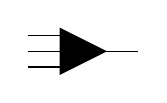
\begin{tikzpicture}[baseline]
				\fill (-0.3,0.3) to (-0.3,-0.3) to (0.3,0);
				\draw[-] (-0.7,0.2) to (-0.3,0.2);
				\draw[-] (-0.7,0) to (-0.3,0);
				\draw[-] (-0.7,-0.2) to (-0.3,-0.2);
				\draw[-] (0.2,0) to (0.7,0);
			\end{tikzpicture} & & 
			\begin{tikzpicture}[baseline]
				\draw[-] (-0.5,0) to (0.5,0);
			\end{tikzpicture} & & 
			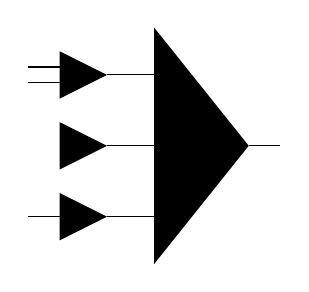
\begin{tikzpicture}[baseline]
				\fill (-1.2,1.2) to (-1.2,0.6) to (-0.6,0.9);
				\fill (-1.2,0.3) to (-1.2,-0.3) to (-0.6,0);
				\fill (-1.2,-1.2) to (-1.2,-0.6) to (-0.6,-0.9);
				\fill (0,1.5) to (0,-1.5) to (1.2,0);
				\draw[-] (-1.6,1) to (-1.2,1);
				\draw[-] (-1.6,0.8) to (-1.2,0.8);
				\draw[-] (-1.6,-0.9) to (-1.2,-0.9);
				\draw[-] (-0.6,0.9) to (0,0.9);
				\draw[-] (-0.6,0) to (0,0);
				\draw[-] (-0.6,-0.9) to (0,-0.9);
				\draw[-] (1.2,0) to (1.6,0);
			\end{tikzpicture} \\
			$n$-ary operation & \quad \quad \quad \quad & Identity & \quad \quad \quad \quad & Operadic multiplication \\
\end{tabular} \end{center}
As an example, if we were to represent some operations pictorially as in the diagram above, then the figure on the right is what is meant by the multiplication $\mu: O(3) \times O(2) \times O(0) \times O(1) \to O(2+0+1)$. Under this interpretation, each of the coherence conditions for an operad represents some obvious fact about how generic $n$-ary operations should interact with one another. For instance, unitality of the identity is simply
\begin{center} \begin{tabular}{ccccc}
			& & & & \\
			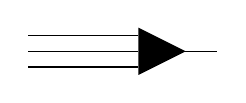
\begin{tikzpicture}[baseline]
				\fill (-0.3,0.3) to (-0.3,-0.3) to (0.3,0);
				\draw[-] (-1.7,0.2) to (-0.3,0.2);
				\draw[-] (-1.7,0) to (-0.3,0);
				\draw[-] (-1.7,-0.2) to (-0.3,-0.2);
				\draw[-] (0.2,0) to  (0.7,0);
			\end{tikzpicture} & &
			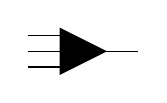
\begin{tikzpicture}[baseline]
				\fill (-0.3,0.3) to (-0.3,-0.3) to (0.3,0);
				\draw[-] (-0.7,0.2) to (-0.3,0.2);
				\draw[-] (-0.7,0) to (-0.3,0);
				\draw[-] (-0.7,-0.2) to (-0.3,-0.2);
				\draw[-] (0.2,0) to  (0.7,0);
			\end{tikzpicture} & &
			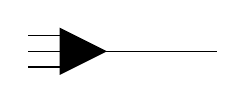
\begin{tikzpicture}[baseline]
				\fill (-0.3,0.3) to (-0.3,-0.3) to (0.3,0);
				\draw[-] (-0.7,0.2) to (-0.3,0.2);
				\draw[-] (-0.7,0) to (-0.3,0);
				\draw[-] (-0.7,-0.2) to (-0.3,-0.2);
				\draw[-] (0.2,0) to  (1.7,0);
			\end{tikzpicture} \\
			& & & & \\
			$\mu( \, x \, ; \, 1, 1, 1 \, )$ & \quad = \quad & $x$ & \quad = \quad & $\mu( \, 1 \, ; \, x \, )$ \\
\end{tabular} \end{center}

As with most mathematical structures, operads naturally form a category, together with a suitable notion of morphisms between operads.

\begin{defn} Given two operads $O, O'$ in a symmetric monoidal category $(C, \otimes, I)$, a \emph{map of operads} between them is a family of maps between their operations which preserve operadic composition. That is, any $f: O \to O'$ is composed of morphisms $f_n : O(n) \to O'(n)$, $n \in \mathbb{N}$ which satisfy
\begin{eq*} \begin{tikzcd}
& I \ar[ddl, "1^O"'] \ar[ddr, "1^{O'}"] & & O(n) \otimes O(k_1) \otimes ... \otimes O(k_n) \ar[dd, "f_n \otimes f_{k_1} \otimes ... \otimes f_{k_n}"'] \ar[r, "\mu^O"] & O(k_1 + ... + k_n) \ar[dd, "f_{k_1 + ... +k_n}"] \\
& & & & \\
O(1) \ar[rr, "f_1"]& & O'(1) & O'(n) \otimes O'(k_1) \otimes ... \otimes O'(k_n) \ar[r, "\mu^{O'}"] & O'(k_1 + ... + k_n)
\end{tikzcd} \end{eq*}
for all $n, k_1, ..., k_n \in \mathbb{N}$. The category of operads and maps of operads in $(C, \otimes, I)$ is denoted $\mathrm{Op}(C)$, though in the case of $\mathrm{Set}$ we will just call it $\mathrm{Op}$. Composition in this category is defined by term-wise composition of families $f_n : O(n) \to O'(n)$, $g_n : O'(n) \to O''(n)$, and the identity morphisms $\mathrm{id}_O : O \to O$ are simply the families $\mathrm{id}_{O(n)}$ from $C$.
\end{defn}

For a far more in depth explanation of operads and their intimate relationship with category theory, see the book `Higher Operads, Higher Categories' \cite{hohc} by Tom Leinster.
 
When we are working with operads in the category of sets, $(\mathrm{Set}, \times, 1)$, the objects $O(n)$ genuinely are collections of elements, with a distinguished identity $1 \in O(1)$. However, these elements still do not have to be operations in any way other than that they satisfy \cref{opdef}, as we will see in the following examples.

\begin{namedexample}[(The symmetric operad)]
There is an operad in $\mathrm{Set}$ whose sets of operations $\mathrm{S}(n)$ are the underlying sets of the symmetric groups $\mathrm{S}_n$. The identity element of this \emph{symmetric operad} $\mathrm{S}$ is the identity permutation of a single object, $e_1 \in \mathrm{S}_1$, and the operadic multiplication is defined in the following way:
\begin{itemize}
\item First, there exist maps $\otimes : \mathrm{S}_m \times \mathrm{S}_n \to \mathrm{S}_{m+n}$ called the \emph{direct sum} or \emph{block sum} of permutations. For any $\sigma \in \mathrm{S}_m$ and $\tau \in \mathrm{S}_n$, these are given by
\begin{eq*} (\sigma \otimes \tau)(i) \quad = \quad \begin{cases}
								\quad \sigma(i) & \quad 1 \le i \le m \\
								\quad \tau(i-m) +m & \quad m+1 \le i \le m+n
							\end{cases}
\end{eq*}
As the name suggests, this direct sum is usually denote by the symbol $\oplus$, but we will stick with $\otimes$ so that our notation here matches all of the other tensor products we will see throughout this paper. Also, notice that the value of these direct sums in general are determined by those specific cases where one of the inputs is an identity permutation:
\begin{eq*} \sigma \otimes \tau \quad = \quad (\sigma \otimes e_n) \cdot (e_m \otimes \tau) \quad = \quad (e_m \otimes \tau) \cdot (\sigma \otimes e_n) \end{eq*}
\item Next, we'll define functions $( \, \_ \, )_{(k_1, ..., k_n)} : \mathrm{S}_n \to \mathrm{S}_{k_1 + ... + k_n}$ for all $n, k_1, ..., k_n \in \mathbb{N}$. These will act by taking a $\sigma$ which permutes $n$ individual objects and sending it onto a $\sigma_{(k_1, ..., k_n)}$ that permutes $n$ blocks of objects of size $k_1, ..., k_n$ in the same way. More concretely, if $k_1 + ... + k_{i-1} < j \le k_1 + ... + k_i$ then
\begin{eq*} \sigma_{(k_1, ..., k_n)}(j) \quad = \quad j - k_1 - ... - k_{i-1} + k_{\sigma^{-1}(1)} + ... + k_{\sigma^{-1}( \, \sigma(i) -1 \, )} \end{eq*}
\item Finally, the multiplication maps $\mu: \mathrm{S}_n \times \mathrm{S}_{k_1} \times ... \times \mathrm{S}_{k_n} \to \mathrm{S}_{k_1 + ... + k_n}$ are given by
\begin{eq*} \begin{array}{rrl} 
			\mu(\sigma; \tau_1, ..., \tau_n) & := & \sigma_{(k_1, ..., k_n)} \cdot (\tau_1 \otimes ... \otimes \tau_n) \\
			& = & (\tau_{\sigma^{-1}(1)} \otimes ... \otimes \tau_{\sigma^{-1}(n)}) \cdot \sigma_{(k_1, ..., k_n)}
		\end{array}
\end{eq*}
In other words, the operadic multiplication of permutations comes from both permutating objects within distinct blocks and also permuting the blocks themselves.
\end{itemize}

If we decide to represent elements of the symmetric operad pictorially --- for example as strings which cross over another according to the appropriate permutation --- then both $\sigma \otimes \tau$ and $\sigma_{(k_1, ..., k_n)}$ have rather nice interpretations. 
\begin{center} \begin{tabular}{ccccc}
			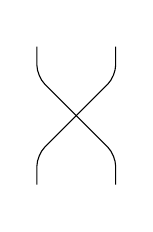
\begin{tikzpicture}[baseline]
				\node(x1) at (-0.5,1){};
				\node(y1) at (0.5,1){};	
				\node(y2) at (-0.5, -1){};
				\node(x2) at (0.5, -1){};
       				\draw[rounded corners](x1.south) to (-0.5,0.5) to (0.5,-0.5) to (x2.north);
				\draw[rounded corners](y1.south) to (0.5, 0.5) to (-0.5, -0.5) to (y2.north);		
			\end{tikzpicture} & \quad $\bigotimes$ \quad \quad &
			\begin{tikzpicture}[baseline]
				\node(x1) at (-0.5,1){};
				\node(y1) at (0.5,1){};	
				\node(x2) at (-0.5, -1){};
				\node(y2) at (0.5, -1){};
				\draw[rounded corners](x1.south) to (x2.north);	
       				\draw[rounded corners](y1.south) to (y2.north);	
			\end{tikzpicture} & \quad $=$ \quad \quad &
			\begin{tikzpicture}[baseline]
				\node(x1) at (-1.5,1){};	
				\node(y1) at (-0.5,1){};
				\node(y2) at (-1.5, -1){};
				\node(x2) at (-0.5, -1){};
				\node(x'1) at (0.5,1){};
				\node(y'1) at (1.5,1){};
				\node(x'2) at (0.5, -1){};
				\node(y'2) at (1.5, -1){};
       				\draw[rounded corners](x1.south) to (-1.5,0.5) to (-0.5,-0.5) to (x2.north);	
				\draw[rounded corners](y1.south) to (-0.5, 0.5) to (-1.5, -0.5) to (y2.north);
				\draw[rounded corners](x'1.south) to (x'2.north);	
       				\draw[rounded corners](y'1.south) to (y'2.north);	
			\end{tikzpicture} \\
			$\sigma$ & & $\tau$ & & $\sigma \otimes \tau$
\end{tabular} \end{center}
The direct sum of two permutations is just the result of placing two permutations `next to' each other, as above, and block permutations are given by expanding each string into some number of parallel strings:
\begin{center} \begin{tabular}{ccc}
			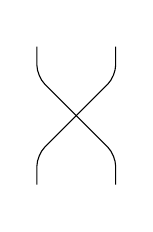
\begin{tikzpicture}[baseline]
				\node(x1) at (-0.5,1){};
				\node(y1) at (0.5,1){};	
				\node(y2) at (-0.5, -1){};
				\node(x2) at (0.5, -1){};
       				\draw[rounded corners](x1.south) to (-0.5,0.5) to (0.5,-0.5) to (x2.north);
				\draw[rounded corners](y1.south) to (0.5, 0.5) to (-0.5, -0.5) to (y2.north);		
			\end{tikzpicture} & \quad $\mapsto$ \quad \quad &
			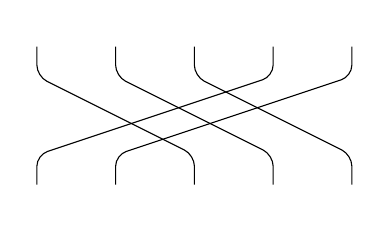
\begin{tikzpicture}[baseline]
				\node(x1) at (-2,1){};
				\node(x'1) at (-1,1){};
				\node(x''1) at (0,1){};
				\node(y1) at (1,1){};	
				\node(y'1) at (2,1){};
				\node(y2) at (-2, -1){};
				\node(y'2) at (-1, -1){};
				\node(x2) at (0, -1){};
				\node(x'2) at (1, -1){};
				\node(x''2) at (2, -1){};
       				\draw[rounded corners](x1.south) to (-2,0.5) to (0,-0.5) to (x2.north);
       				\draw[rounded corners](x'1.south) to (-1,0.5) to (1,-0.5) to (x'2.north);
       				\draw[rounded corners](x''1.south) to (0,0.5) to (2,-0.5) to (x''2.north);
				\draw[rounded corners](y1.south) to (1, 0.5) to (-2, -0.5) to (y2.north);
				\draw[rounded corners](y'1.south) to (2, 0.5) to (-1, -0.5) to (y'2.north);	
			\end{tikzpicture} \\
			$\sigma$ & & $\sigma_{(3, 2)}$
\end{tabular} \end{center}
With a little work, we can actually replace the functions $( \, \_ \, )_{(k_1, ..., k_n)}$ with an explicit combination of group multiplication and tensor product. This is due to basic fact about the symmetric groups $\mathrm{S}_n$, which is that they possess a presentation in terms of the \emph{elementary transpositions} $(i \,\,\,  i+1)$.

\begin{lem} \label{sympres} The group $\mathrm{S}_n$ is generated by the permutations $(1 \, 2), ..., (n-1 \, \, \, n)$, subject to the relations
\begin{eq*} \begin{array}{rclll}
			(i \, \, \, i+1)^2 & = & e & & \\
			(i-1 \, \, \, i)(i \, \, \, i+1)(i-1 \, \, \, i) & = & (i \, \, \, i+1)(i-1 \, \, \, i)(i \, \, \, i+1) & & \\
			(i \, \, \, i+1)(j \, \, \, j+1) & = & (j \, \, \, j+1)(i \, \, \, i+1), & & i+1 < j
		\end{array}
\end{eq*}
\end{lem}

Thus if $\sigma \in \mathrm{S}_n$ is a permutation with a decomposition $\sigma = \sigma_m \cdot ... \cdot \sigma_1 $ in terms of elementary transpositions $\sigma_i \in \mathrm{S}_n$, we can break down the block permutation $\sigma_{(k_1, ..., k_n)}$ into the $m$ `elementary block transpositions' $(\sigma_i)_{(k_1, ..., k_n)}$:
\begin{eq*} \begin{array}{rll}
			\sigma_{(k_1, ..., k_n)}(j) & = & j - k_1 - ... - k_{i-1} + k_{\sigma^{-1}(1)} + ... + k_{\sigma^{-1}( \, \sigma(i) -1 \, )} \\
			& = & j - k_1 - ... - k_{i-1} \\
			& & + \, k_{\sigma_1^{-1}(1)} + ... + k_{\sigma_1^{-1}( \, \sigma_1(i) -1 \, )} \\
			& & -  \, k_{\sigma_1^{-1}(1)} - ... - k_{\sigma_1^{-1}( \, \sigma_1(i) -1 \, )} \\
			& & + \, k_{(\sigma_2 \sigma_1)^{-1}(1)} + ... + k_{(\sigma_2 \sigma_1)^{-1}( \, \sigma_2\sigma_1(i) -1 \, )} \\
			& & \vdots \\
			& & - \,  k_{(\sigma_{m-1}...\sigma_1^{-1}(1)} - ... - k_{(\sigma_{m-1}...\sigma_1)^{-1}( \, \sigma_{m-1}...\sigma_1(i) - 1 \, )} \\
			& & + \, k_{(\sigma_m...\sigma_1)^{-1}(1)} + ... + k_{(\sigma_m...\sigma_1)^{-1}( \, \sigma_m...\sigma_1(i) - 1 \, )} \\
			& = & \big( \, (\sigma_m)_{(k_1, ..., k_n)} \cdot ... \cdot (\sigma_1)_{(k_1, ..., k_n)} \, \big)(j)
		\end{array}
\end{eq*}
However, since elementary transpositions only really permute two objects, they can be written as a block sum in the operad $\mathrm{S}$ involving the sole transposition of $\mathrm{S}_2$, plus some number of identity permutations.
\begin{eq*} (i \, \, \, i+1) \quad = \quad e_{i-1} \otimes (1 \, 2) \otimes e_{n-i-1} \end{eq*}
This means that the elementary block transpositions are
\begin{eq*} \begin{array}{rll}
			(i \, \, \,  i+1)_{(k_1, ..., k_n)} & = & \quad (e_{i-1} \otimes (1 \, 2) \otimes e_{n-i-1})_{(k_1, ..., k_n)} \\
			& = & e_{k_1 + ... k_{i-1}} \otimes (1 \, 2)_{(k_i, k_{i+1})} \otimes e_{k_{i+1} + ... k_n}
		\end{array}
\end{eq*}
So all we need to know to fully understand the functions $( \, \_ \, )_{(k_1, ..., k_n)}$ are the values they take on the transposition $(1 \, 2)$. These can be defined recursively, via
\begin{eq*} \begin{array}{lclclcl}
			(1 \, 2)_{(0, n)} & = & e_n, & \quad \quad & (1 \, 2)_{(m+m', n)} & = & \big( \, (1 \, 2)_{(m, n)} \otimes e_{m'} \, \big) \cdot \big( \, e_m \otimes (1 \, 2)_{(m', n)} \, \big), \\
			(1 \, 2)_{(m, 0)} & = & e_m, & \quad \quad & (1 \, 2)_{(m, n+n')} & = & \big( \, e_n \otimes (1 \, 2)_{(m, n')} \, \big) \cdot \big( \, (1 \, 2)_{(m, n)} \otimes e_{n'} \, \big) \\
			(1 \, 2)_{(1,1)} & = & (1 \, 2), & & & &		
		\end{array}
\end{eq*}
which all follow from the definition of $( \, \_ \, )_{(k_1, ..., k_n)}$. Therefore all $\sigma_{(k_1, ..., k_n)}$ and hence all $\mu(\sigma; \tau_1, ..., \tau_n)$ can be expressed in terms of group multiplication $\cdot$ and direct sum $\otimes$, and the elementary permutations which constitute $\sigma, \tau_1, ..., \tau_n$.
\end{namedexample}

Something very important to notice about the symmetric operad is that while its sets of operations $\mathrm{S}_n$ are groups, it is \emph{not} an operad in the category of groups, because the operadic multiplication we have just outlined is not a group homomorphism. If it were, then it would obey
\begin{eq*} \mu(\sigma; \tau_1, ..., \tau_n) \cdot \mu(\sigma'; \tau'_1, ..., \tau'_n) \quad = \quad \mu( \, \sigma\sigma' \, ; \, \tau_1\tau'_1, ..., \tau_n\tau'_n \, ) \end{eq*}
for all $\sigma, \sigma' \in \mathrm{S}_n$, $\tau_i, \tau'_i \in \mathrm{S}_{k_i}$, but this is clearly false. As a counterexample, consider the fairly simple case
\begin{eq*} \begin{array}{rcccccl}
			\mu\big( \, (1 \, 2) \, ; \, e_2, e_1 \, \big) & = & (1 \, 2)_{(2, 1)} \cdot (e_2 \otimes e_1) & = & (1 \, 2 \, 3) \cdot e_3 & = & (1 \, 2 \, 3) \\
			\mu\big( \, e_2 \, ; \, (1 \, 2), e_1 \, \big) & = & {(e_2)}_{(2, 1)} \cdot \big(\, (1 \, 2) \otimes e_1 \, \big) & = & e_3 \cdot (1 \, 2) & = & (1 \, 2) \\
			\mu\big( \,  (1 \, 2) \, ; \, (1 \, 2), e_1 \, \big) & = & (1 \, 2)_{(2, 1)} \cdot \big(\, (1 \, 2) \otimes e_1 \, \big) & = & (1 \, 2 \, 3) \cdot (1 \, 2) & &
		\end{array}
\end{eq*}
Then we have
\begin{eq*} \mu\big( \, e_2 \, ; \, (1 \, 2), e_1 \, \big) \cdot \mu\big( \, (1 \, 2) \, ; \, e_2, e_1 \, \big) \quad = \quad (1 \, 2) \cdot (1 \, 2 \, 3) \end{eq*}
which is \emph{not} the same as
\begin{eq*} \mu\big( \, e_2 \cdot (1 \, 2) \, ; \, (1 \, 2) \cdot e_2 , \, e_1 \cdot e_1 \, \big) \quad = \quad \mu\big( \,  (1 \, 2) \, ; \, (1 \, 2), e_1 \, \big) \quad = \quad (1 \, 2 \, 3) \cdot (1 \, 2) \end{eq*}
At first this seems like pretty strange behaviour. After all, the symmetric groups play a central role in the theory of groups, so it would be reasonable to assume that their operad would be similarly crucial for the theory of group operads. But $\mathrm{S}$ is not the only family of groups whose operad is fundamentally set related.

\begin{namedexample}[(The braid operad)]\label{braidop}
The \emph{braid groups} $B_n$ are the family of groups that result from taking the symmetric groups and removing the requirement that everything needs to be self-inverse. That is, the group $B_n$ has a presentation on some \emph{elementary braids} $b_1, ..., b_{n-1}$, given by the relations
\begin{eq*} b_i b_{i+1} b_i \, = \, b_{i+1} b_i b_{i+1}, \quad \quad \quad \quad \quad b_i b_j \, = \, b_j b_i, \quad i+1 < j \end{eq*}
As might be expected, the underlying sets of these groups also form an operad in $\mathrm{Set}$ known as the \emph{braid operad} $B$, and they do so in a way directly analogous to the operad $\mathrm{S}$. That is, the identity element of $B$ is $e_1 \in B_1$, and the operadic multiplication is constructed as follows:
\begin{itemize}
\item Tensor products $\otimes : B_m \times B_n \to B_{m+n}$ are determined by setting 
\begin{eq*} x \otimes y \quad = \quad (x \otimes e_n) \cdot (e_m \otimes y) \quad = \quad (e_m \otimes x) \cdot (y \otimes e_n) \end{eq*}
for all $x \in B_m$, $y \in B_n$, and also
\begin{eq*} b_i \quad = \quad e_{i-1} \otimes b \otimes e_{n-i-1} \end{eq*}
for any elementary braid $b_i \in B_n$, where $b$ is the only elementary braid in $B_2$.
\item The functions $( \, \_ \, )_{(k_1, ..., k_n)} : B_n \to B_{k_1 + ... + k_n}$ are first defined recursively on the elementary braid $b \in B_2$ by
\begin{eq*} \begin{array}{rclcrcl}
			b_{(0, n)} & = & e_n, & \quad \quad & b_{(m+m', n)} & = & (b_{(m, n)} \otimes e_{m'}) \cdot (e_m \otimes b_{(m', n)}) \\
			b_{(m, 0)} & = & e_m, & \quad \quad & b_{(m, n+n')} & = & (e_n \otimes b_{(m, n')}) \cdot (b_{(m, n)} \otimes e_{n'}) \\
			b_{(1,1)} & = & b & & & &				
		\end{array}
\end{eq*}
then on arbitrary elementary braids $b_i \in B_n$ via
\begin{eq*} (b_i)_{(k_1, ..., k_n)} \quad = \quad e_{k_1 + ... k_{i-1}} \otimes b_{(k_i, k_{i+1})} \otimes e_{k_{i+1} + ... k_n} \end{eq*}
and finally on all elements of the braid groups by using their presentation in terms of the $b_i$,
\begin{eq*} \begin{array}{rll}
			x & = & b_{i_m} \cdot ... \cdot b_{i_1} \\
			\implies \quad x_{(k_1, ..., k_n)} & = & (b_{i_m})_{(k_1, ..., k_n)} \cdot ... \cdot (b_{i_1})_{(k_1, ..., k_n)} 
		\end{array}
\end{eq*}
\item Then as in the symmetric case, the multiplication maps $\mu: B_n \times B_{k_1} \times ... \times B_{k_n} \to B_{k_1 + ... + k_n}$ are just
\begin{eq*} \mu(x; y_1, ..., y_n) \quad := \quad x_{(k_1, ..., k_n)} \cdot (y_1 \otimes ... \otimes y_n) \end{eq*}
\end{itemize}

These operations are exactly what they need to be in order for them to possess the same pictorial representations as the operations in $\mathrm{S}$, but with actual braids replacing simple crossings. That is, the tensor product $x \otimes y$ is the braids $x$ and $y$ laid side-by-side,
\begin{center} \begin{tabular}{ccccc}
			\begin{tikzpicture}[baseline]
				\node(x1) at (-0.5,1){};
				\node(y1) at (0.5,1){};	
				\node(y2) at (-0.5, -1){};
				\node(x2) at (0.5, -1){};
				\node(b) at (0,0)[circle,fill=white]{};
       				\draw[rounded corners](x1.south) to (-0.5,0.5) to (0.5,-0.5) to (x2.north);
				\begin{pgfonlayer}{bg}
				\draw[rounded corners](y1.south) to (0.5, 0.5) to (-0.5, -0.5) to (y2.north);
    				\end{pgfonlayer}	
			\end{tikzpicture} & \quad $\bigotimes$ \quad \quad &
			\begin{tikzpicture}[baseline]
				\node(x1) at (-0.5,1){};
				\node(y1) at (0.5,1){};	
				\node(x2) at (-0.5, -1){};
				\node(y2) at (0.5, -1){};
				\draw[rounded corners](x1.south) to (x2.north);	
       				\draw[rounded corners](y1.south) to (y2.north);	
			\end{tikzpicture} & \quad $=$ \quad \quad &
			\begin{tikzpicture}[baseline]
				\node(x1) at (-1.5,1){};	
				\node(y1) at (-0.5,1){};
				\node(y2) at (-1.5, -1){};
				\node(x2) at (-0.5, -1){};
				\node(b) at (-1,0)[circle,fill=white]{};
				\node(x'1) at (0.5,1){};
				\node(y'1) at (1.5,1){};
				\node(x'2) at (0.5, -1){};
				\node(y'2) at (1.5, -1){};
       				\draw[rounded corners](x1.south) to (-1.5,0.5) to (-0.5,-0.5) to (x2.north);	
				\begin{pgfonlayer}{bg}
				\draw[rounded corners](y1.south) to (-0.5, 0.5) to (-1.5, -0.5) to (y2.north);
    				\end{pgfonlayer}
				\draw[rounded corners](x'1.south) to (x'2.north);	
       				\draw[rounded corners](y'1.south) to (y'2.north);	
			\end{tikzpicture} \\
			$x$ & & $y$ & & $x \otimes y$
\end{tabular} \end{center}
and the `block braids' are multiple strings braided together in parallel,
\begin{center} \begin{tabular}{ccc}
			\begin{tikzpicture}[baseline]
				\node(x1) at (-0.5,1){};
				\node(y1) at (0.5,1){};	
				\node(y2) at (-0.5, -1){};
				\node(x2) at (0.5, -1){};
				\node(b) at (0,0)[circle,fill=white]{};
       				\draw[rounded corners](x1.south) to (-0.5,0.5) to (0.5,-0.5) to (x2.north);
				\begin{pgfonlayer}{bg}
				\draw[rounded corners](y1.south) to (0.5, 0.5) to (-0.5, -0.5) to (y2.north);
    				\end{pgfonlayer}		
			\end{tikzpicture} & \quad $\mapsto$ \quad \quad &
			\begin{tikzpicture}[baseline]
				\node(x1) at (-2,1){};
				\node(x'1) at (-1,1){};
				\node(x''1) at (0,1){};
				\node(y1) at (1,1){};	
				\node(y'1) at (2,1){};
				\node(y2) at (-2, -1){};
				\node(y'2) at (-1, -1){};
				\node(x2) at (0, -1){};
				\node(x'2) at (1, -1){};
				\node(x''2) at (2, -1){};
				\node(b1) at (-0.8,-0.1)[circle,fill=white]{};
				\node(b2) at (-0.2,0.1)[circle,fill=white]{};
				\node(b3) at (0.4,0.3)[circle,fill=white]{};
				\node(b4) at (-0.4,-0.3)[circle,fill=white]{};
				\node(b5) at (0.2,-0.1)[circle,fill=white]{};
				\node(b6) at (0.8,0.1)[circle,fill=white]{};
       				\draw[rounded corners](x1.south) to (-2,0.5) to (0,-0.5) to (x2.north);
       				\draw[rounded corners](x'1.south) to (-1,0.5) to (1,-0.5) to (x'2.north);
       				\draw[rounded corners](x''1.south) to (0,0.5) to (2,-0.5) to (x''2.north);
				\begin{pgfonlayer}{bg}
				\draw[rounded corners](y1.south) to (1, 0.5) to (-2, -0.5) to (y2.north);
				\draw[rounded corners](y'1.south) to (2, 0.5) to (-1, -0.5) to (y'2.north);
    				\end{pgfonlayer}	
			\end{tikzpicture} \\
			$x$ & & $x_{(3, 2)}$
\end{tabular} \end{center}
\end{namedexample}

\section{Action operads}

It is not hard to see that the symmetric and braided operads both share certain features which are not otherwise common among operads of sets. This fact has been noticed by several different authors, each of whom proposed a slightly different definition and terminology for these sorts of structures. While older treatments exist --- see for example \cite{ribbon1} and \cite{groupop} --- in this paper we will be following the conventions laid out in \cite{ogge}, since they are the most general.

\begin{defn} \label{actop} An \emph{action operad} $(G, \pi)$ consists of 
\begin{itemize}
\item an operad $G$ in the category of sets, whose $G(n)$ are also all groups
\item a map of operads $\pi : G \to \mathrm{S}$ whose components $\pi_n : G(n) \to \mathrm{S}_n$ are also group homomorphisms
\end{itemize}
where the operadic multiplication of $G$ and the group multiplication of the $G(n)$ are linked via the map $\pi$ in the following way:
\begin{eq*} \mu( \, gg' \, ; \, h_1 h'_1, ...,  h_n h'_n \, ) \quad = \quad \mu(g; h_{\pi(g')^{-1}(1)}, ..., h_{\pi(g')^{-1}(n)}) \cdot \mu(g'; h'_1, ..., h'_n) \end{eq*}
\end{defn}

The element $\pi(g)$ is called the \emph{underlying permutation} of $g$, and as we can see the role it plays is to permute the inputs of an operadic multiplication when two of them are multiplied as group elements. This is exactly the behaviour we observed before with the symmetric operad; for instance, recalling our previous example we see that what we should have had was
\begin{eq*} \begin{array}{rclllll}
			\mu\big( \, (1 \, 2) \, ; \, e_1, e_2 \, \big) & = & (1 \, 2 \, 3) & & & & \\
			\mu\big( \, e_2 \, ; \, e_1, (1 \, 2) \, \big) & = & {(e_2)}_{(1, 2)} \cdot \big(\, e_1 \otimes (1 \, 2) \, \big) & = & e_3 \cdot (2 \, 3) & = & (2 \, 3) \\
			\mu\big( \,  (1 \, 2) \, ; \, (1 \, 2), e_1 \, \big) & = & (1 \, 2 \, 3) \cdot (1 \, 2) & & & &
		\end{array}
\end{eq*}
\begin{eq*} \begin{array}{rll}
			\implies \mu\big( \, e_2 \, ; \, (1 \, 2), e_1 \, \big) \cdot \mu\big( \, (1 \, 2) \, ; \, e_2, e_1 \, \big) & = & (2 \, 3) \cdot (1 \, 2 \, 3) \\
			& = &  (1 \, 2 \, 3) \cdot (1 \, 2) \\
			& = & \mu\big( \,  (1 \, 2) \, ; \, (1 \, 2), e_1 \, \big) \\
			& = & \mu\big( \, e_2 \cdot (1 \, 2) \, ; \, (1 \, 2) \cdot e_2 , \, e_1 \cdot e_1 \, \big)
		\end{array}
\end{eq*}
The effect that this has on the map $\mu$ also mirrors the way that we had to define operadic multiplication for $\mathrm{S}$ and $B$ in stages. Specifically, if for any action operad $G$ we define
\begin{eq*} g_{(k_1, ..., k_n)} \, := \, \mu(g; e_{k_1}, ..., e_{k_n}), \quad \quad \quad g_1 \otimes ... \otimes g_n \, := \, \mu(e_n; g_1, ..., g_n) \end{eq*}
then it follows from \cref{actop} that
\begin{eq*} \begin{array}{rll}
			\mu( \, g \, ; \, h_1, ..., h_n \, ) & = & \mu( \, g \cdot e_n \, ; \, e_{k_1} \cdot h_1, ..., e_{k_n} \cdot h_n \, ) \\
			& = & \mu( \, g \, ; \, e_{\pi(e_n)^{-1}(k_1)} ..., e_{\pi(e_n)^{-1}(k_1)} \, ) \cdot \mu( \, e_n \, ; \, h_1, ..., h_n \, ) \\
			& = & \mu( \, g \, ; \, e_{k_1} ..., e_{k_1} \, ) \cdot \mu( \, e_n \, ; \, h_1, ..., h_n \, ) \\
			& = & g_{(k_1, ..., k_n)} \cdot (h_1 \otimes ... \otimes h_n)
		\end{array}
\end{eq*}
for all $g \in G(n)$, $h_i \in G(k_i)$, $n, k_1, ..., k_n \in \mathbb{N}$. 

Now we can also see the reason why we chose the tensor product notation for the operation $\mu(e_n; \_, ..., \_)$ before. Just like the tensor product of a monoidal category, the definition of this $\otimes$ in $G$ immediately implies an interchange law:
\begin{eq*} \begin{array}{rll}
			(g \cdot g') \otimes (h \cdot h') & = & \mu( \, e_2 \, ; \, gg', \, hh' \, ) \\
			& = & \mu(e_2; g, h) \cdot \mu(e_2; g', h')\\
			& = & (g \otimes h) \cdot (g' \otimes h')
		\end{array}
\end{eq*}
This interaction between the operad and group structures of $G$ places some restrictions on which groups we may build action operads from. One such consequence that we will refer to in later chapters is the following: 

\begin{lem} \label{G0abel} For any action operad $G$, the group $G(0)$ is abelian.  
\end{lem}
\begin{proof}
This lemma is an example of the classic Eckmann-Hilton argument, first put forth in \cite{eckhil}. The idea is that if a set is equipped with two binary operations which obey some form of interchange, and both of them possess the same unit element $e$, then they are in reality a single, commutative operation.

In the case of $G(0)$, we know that it is closed under group multiplication $\cdot$, and the unit of this is the identity element $e_0$. But the operadic multiplication of $G$ includes a map
\begin{eq*} \mu_{n;0,...,0} \, : \, G(n) \times G(0) \times ... \times G(0) \, \longrightarrow \, G(0+...+0) \, = \, G(0) \end{eq*}
which means that tensor products of elements in $G(0)$,
\begin{eq*} g_1 \otimes ... \otimes g_n \quad = \quad \mu_{n;0,...,0}(e_n; g_1, ..., g_n) \end{eq*}
are also in $G(0)$. This $\otimes$ has unit $e_0$ as well; since $(e_2;e_1,e_0)$ is the identity of $G(2)\times G(1)\times G(0)$, the operadic associativity, unitality, and group homomorphism property $\mu$ gives
\begin{eq*} \begin{array}{rll}
			g \otimes e_0 & = & \mu(e_2; g, e_0) \\
			& = & \mu\big( \, e_2 \, ; \, \mu(e_1;g), \, \mu(e_0; -) \, \big) \\
			& = & \mu\big( \, \mu(e_2;e_1,e_0) \, ; \, g \, \big) \\
			& = & \mu(e_1;g) \\
			& = & g
		\end{array}
\end{eq*}
and likewise for $e_0 \otimes g = g$. Moreover, we've just seen that the group multiplication and tensor product of $G$ obey an interchange law. Therefore we can apply the Eckmann-Hilton argument: for any $g, h \in G(0)$,
\begin{eq*} g \otimes h \quad = \quad (g \cdot e_0) \otimes (e_0 \cdot h) \quad = \quad (g \otimes e_0) \cdot (e_0 \otimes h) \quad = \quad g \cdot h \end{eq*}
and also
\begin{eq*} h \otimes g \quad = \quad (e_0 \cdot h) \otimes (g \cdot e_0) \quad = \quad (e_0 \otimes g) \cdot (h \otimes e_0) \quad = \quad g \cdot h \end{eq*}
In other words, tensor product and group multiplication coincide on $G(0)$, and are commutative, so that $G(0)$ is an abelian group.
\end{proof}

Much like standard operads, we can pair action operads with a natural notion of maps between them in order to form a category.

\begin{defn} Given action operads $G, G'$, a \emph{map of action operads} $f: G \to G'$ is a map of operads in $\mathrm{Set}$ whose components $f_n : G(n) \to G'(n)$ are all group homomorphisms, and which preserve all underlying permutations:
\begin{eq*} \begin{tikzcd}
G(n) \ar[rr, "f_n"] \ar[ddr, "\pi^G"'] & & G'(n) \ar[ddl, "\pi^{G'}"] \\
& & \\
& \mathrm{S}_n &
\end{tikzcd} \end{eq*}
The identity maps $\mathrm{id}_G : G \to G$ and the composites of action operad maps $g \circ f : G \to G' \to G''$ in $\mathrm{Op}$ are all well-defined maps of action operads themselves, and so together these constitute a category of action operads and their maps, called $\mathrm{AOp}$.
\end{defn}

There are a couple of operads which trivially have the structure of an action operad. First we have the \emph{terminal operad} $\mathrm{T}$, which has a single operation for each arity, so that $\mathrm{T}(n) = \{ e_n \}$. Each of these sets can be seen as the trivial group, and it follows from this that the $\pi^{\mathrm{T}} : \mathrm{T}(n) \to \mathrm{S}_n$ must be the respective zero maps, the terminal homomorphisms in the category of groups. The action operad condition is then
\begin{eq*} \mu(e_n; e_{k_1}, ..., e_{k_n}) \cdot \mu(e_n; e_{k_1}, ..., e_{k_n}) \quad = \quad \mu(e_n; e_{k_1}, ..., e_{k_n}) \end{eq*}
which is really just
\begin{eq*} e_{k_1 + ... + k_n} \cdot e_{k_1 + ... + k_n} \, = \, e_{k_1 + ... + k_n} \end{eq*}
and hence is trivially true. As its name suggests, the terminal operad is the terminal object in the category $\mathrm{Op}$, but it is also the \emph{initial} object in $\mathrm{AOp}$. This is because for any other $G$ in the category of action operads, the zero homomorphisms $\mathrm{T}(n) \to G(n)$ define the unique map of operads $f: \mathrm{T} \to G$.

On the other hand, the symmetric operad $\mathrm{S}$ itself functions as the terminal object in $\mathrm{AOp}$. Its action operad structure is just given by the standard group multiplications on the $\mathrm{S}_n$, with the identity maps $\mathrm{id}_{\mathrm{S}_n} : \mathrm{S}_n \to \mathrm{S}_n$ functioning as its $\pi_n$. To see terminality, notice that for any other action operad $G$ a valid morphism $f: G \to \mathrm{S}$ in $\mathrm{AOp}$ must obey
\begin{eq*} \pi^{\mathrm{S}} \circ f \, = \, \pi^{G} \quad \implies \quad f \, = \, \pi^{G} \end{eq*}
Thus there is only one map of action operads $G \to \mathrm{S}$: the very underlying permutation structure used to define $G$ in the first place.

There are more interesting examples of action operads we can look at too. For instance, we know that the braid groups $B_n$ have the same presentation as the symmetric groups, except without the relations $b_i^2 = e$. Thus if we take their quotients by these relations we will obtain a sequence of homomorphisms $B_n \to \mathrm{S}_n$, each sending $b_i \mapsto (i \, \, \, i+1)$. This provides a natural way to describe the underlying permutation of any braid, and indeed choosing these maps to form $\pi^B$ gives a valid way of seeing the braid operad as an action operad. Another example can also be built from the so-called ribbon braid groups.

\begin{defn} For each $n \in \mathbb{N}$, the \emph{ribbon braid group} $RB_n$ is the group whose presentation is the same as that of the braid group $B_n$, except with the addition of $n$ new generators $t_1, ..., t_n$, known as the \emph{twists}. These twists all commute with one other, and also commute with all braids except in the following cases:
\begin{eq*} b_i \cdot t_i \quad = \quad t_{i+1} \cdot b_i, \quad \quad \quad \quad \quad b_i \cdot t_{i+1} \quad = \quad t_i \cdot b_i \end{eq*}
The \emph{ribbon braid operad} $RB$ is then the operad made up of these groups in a way that extends the definition of the braid operad. In other words, the identity is still $e_1 \in RB_1$, and the operadic multiplication is built up in stages in exactly the same ways as in \cref{braidop}, but with some additional rules for dealing with twists. With regards to the tensor product, we have that for any twist $t_i \in RB_n$,
\begin{eq*} t_i \quad = \quad e_{i-1} \otimes t \otimes e_{n-i} \end{eq*}
where $t$ is the sole twist in $RB_1$, and for the `block twists' $t_{(m)}$ we again work recursively:
\begin{eq*} t_{(0)} \, = \, e_n, \quad \quad \quad t_{(m+m')} \quad = \quad (t_{(m)} \otimes t_{(m')}) \cdot b_{(m', m)} \cdot b_{(m, m')} \end{eq*}
\end{defn}

Much as the symmetric groups can be represented by crossings of a collection of strings, and the braid groups by braidings of strings, the ribbon braid groups deal with the ways that one can braid together several flat ribbons, including the ability to twist a ribbon about its own axis by 360 degrees.
\begin{center} \begin{tabular}{ccc}
			\begin{tikzpicture}[baseline]
				\node(xl1) at (-0.7,1){};
				\node(xr1) at (-0.3,1){};
				\node(yl1) at (0.3,1){};
				\node(yr1) at (0.7,1){};
				\node(yl2) at (-0.7, -1){};
				\node(yr2) at (-0.3, -1){};
				\node(xl2) at (0.3, -1){};
				\node(xr2) at (0.7, -1){};
				\node(b) at (0,0)[circle,fill=white, minimum size=0.5cm]{};
       				\draw[rounded corners](xl1.north) to (-0.7,0.5) to (0.3,-0.5) to (xl2.south);
       				\draw[rounded corners](xr1.north) to (-0.3,0.5) to (0.7,-0.5) to (xr2.south);
				\begin{pgfonlayer}{bg}
				\draw[rounded corners](yl1.north) to (0.3, 0.5) to (-0.7, -0.5) to (yl2.south);
				\draw[rounded corners](yr1.north) to (0.7, 0.5) to (-0.3, -0.5) to (yr2.south);
    				\end{pgfonlayer}
				\draw(xl1.north) to (xr1.north);
				\draw(xl2.south) to (xr2.south);
				\draw(yl1.north) to (yr1.north);
				\draw(yl2.south) to (yr2.south);
			\end{tikzpicture} & \quad \quad \quad \quad \quad \quad \quad &
			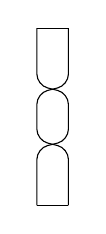
\begin{tikzpicture}[baseline]
				\node(xl1) at (-0.2,1){};
				\node(xr1) at (0.2,1){};	
				\node(xl2) at (-0.2, -1){};
				\node(xr2) at (0.2, -1){};
				\draw[rounded corners](xl1.north) to (-0.2,0.4) to (0.2, 0.3) to (0.2, -0.3) to (-0.2, -0.4) to (xl2.south);	
       				\draw[rounded corners](xr1.north) to (0.2,0.4) to (-0.2, 0.3) to (-0.2, -0.3) to (0.2, -0.4) to (xr2.south);
				\draw(xl1.north) to (xr1.north);
				\draw(xl2.south) to (xr2.south);	
			\end{tikzpicture} \\
			$b$ & & $t$ 
\end{tabular} \end{center}
This operad $RB$ is also clearly an action operad, since we can just define $\pi^{RB} : RB_n \to \mathrm{S}_n$ to act like $\pi^B$ on any braids, at which point the fact that $\pi(t) \in S_1 = \{e_1\}$ will automatically take care of the twists. To learn more about the ribbon braids and their operads, see Natalie Wahl's thesis \cite{ribbon1} on the subject, or her subsequent paper with Paolo Salvatore \cite{ribbon2}.

The fact that the ribbon braid operad seems to contain the whole of the braid operad is the key to easily understanding its operadic structure. We can formalise this kind of relationship in the following way:

\begin{defn} An action operad $G$ is said to be a \emph{sub action operad} of some other action operad $G'$ if for all $n \in \mathbb{N}$ we have
\begin{eq*} G(n) \le G'(n), \quad \quad \quad \mu^{G}(g;h_1, ..., h_n) \, = \, \mu^{G'}(g;h_1, ..., h_n), \quad \quad \quad \pi^{G}(g) \, = \, \pi^{G'}(g) \end{eq*}
\end{defn}

The most important example of sub action operads are those of the symmetric operad, $\mathrm{S}$. This is because \cref{actop} itself makes explicit reference to the symmetric groups, and so every action operad will end up being related to some sub-operad of $\mathrm{S}$:

\begin{defn} For any action operad $G$, the images of the underlying permutation maps $\pi^G_n : G(n) \to \mathrm{S}_n$ naturally form an action operad $\mathrm{im}(\pi^G)$, where
\begin{itemize}
\item the sets of operations are the images of $G$'s sets of operations under the homomorphisms $\pi^G$:
\begin{eq*} \mathrm{im}(\pi^G)(n) \quad := \quad \mathrm{im}(\pi^G_n) \end{eq*}
\item the underlying permutation maps are the evident inclusions:
\begin{eq*} \pi^{\mathrm{im}(\pi^G)}_n \, : \, \mathrm{im}(\pi^G_n) \hookrightarrow \mathrm{S}_n \end{eq*}
\item the operad multiplication is the appropriate restriction of the multiplication of $\mathrm{S}$:
\begin{eq*} \mu^{\mathrm{im}(\pi^G)}( \, g \, ; \, h_1, ..., h_n \, ) \quad := \quad \mu^{\mathrm{S}}( \, g \, ; \, h_1, ..., h_n \, ) \end{eq*}
\end{itemize}
Clearly this $\mathrm{im}(\pi^G)$ is a sub action operad of the symmetric operad $\mathrm{S}$, and so we will call it the \emph{underlying permutation operad} of $G$.
\end{defn} 

For example, consider the action operad $B$ we just saw in \cref{braidop}. For a given $n$, the braid group $B_n$ is generated by $n-1$ elementary braids. But the underlying permutations of these braids are just the $n-1$ elementary transpositions which generate the symmetric group $\mathrm{S}_n$, and so the underlying permutation maps $\pi^{B}_n : B_n \to \mathrm{S}_n$ are all surjective. Thus the underlying permutation operad of $B$ is just the whole symmetric action operad, $\mathrm{im}(\pi^B) = \mathrm{S}$.

It is even easier to see that $\mathrm{S}$ itself will have underlying permutations $\mathrm{S}$, as the maps $\pi^{\mathrm{S}}_n = \mathrm{id} : \mathrm{S}_n \to \mathrm{S}_n$ are obviously surjective. Similarly, the trivial operad $\mathrm{T}$ is also its own underlying permutation action operad, as the image of the homomorphisms $\pi^{\mathrm{T}}_n : \{ e \} \to \mathrm{S}_n$ are trivial. Faced with rather dull examples like these, it might be tempting to try and construct some new action operads with more exotic underlying permutations, like maybe the alternating groups $\mathrm{A}_n \subset \mathrm{S}_n$. But it turns out that this is not possible; when it come to their underlying permutation operad, action operads come in exactly two flavours, as seen in \cite{groupop}.

\begin{defn} Let $G$ be an action operad where $\mathrm{im}(\pi)(n)$ is the trivial group for each $n \in \mathbb{N}$. Then we say that $G$ is \emph{non-crossed}, since its operad multiplication will be a true group homomorphism:
\begin{eq*} \begin{array}{rll}
			\mu( \, gg' \, ; \, h_1 h'_1, ..., h_n h'_n \, ) & = & \mu( \, g \, ; \, h_{\pi(g')^{-1}(1)}, ..., h_{\pi(g')^{-1}(n)} \, ) \mu( \, g' \, ; \, h'_1, ..., h'_n \, ) \\
			& = & \mu( \, g \, ; \, h_1, ..., h_n \, ) \mu( \, g' \, ; \, h'_1, ..., h'_n \, ) \\
		\end{array}
\end{eq*}
Likewise, a \emph{crossed} action operad will refer to any that has a non-trivial underlying permutation operad.
\end{defn}

\begin{lem}\label{surjortriv} An action operad $G$ is crossed if and only if it has surjective underlying permutation maps $\pi_n : G(n) \to \mathrm{S}_n$. In other words, the underlying permutations operad of $G$ must be either the trivial operad $\mathrm{T}$ or the symmetric operad $\mathrm{S}$.
\end{lem}
\begin{proof}
Let $\mathrm{im}(\pi)$ be the underlying permutation operad of $G$, and let us assume that $G$ is crossed, so that $\mathrm{im}(\pi)$ is not the trivial operad. This means that for some natural number $n$, the $n$-ary operations of $\mathrm{im}(\pi)$ include at least one permutation $\sigma$ which is not the identity element of the relevant symmetric group $\mathrm{S}_n$. Put another way, there must be some $\sigma$ and some $1 \le i \le n$ for which $\sigma(i) \neq i$. But now consider evaluating the expression
\begin{eq*} \mu^{\mathrm{im}(\pi)}( \, \sigma \, ; \, e_0, ..., e_0, e_1, e_0, ...., e_0, e_1, e_0, ..., e_0 \, ) \end{eq*}
where the $e_1$'s above are appearing in the $i$th and $\sigma(i)$th coordinates, which we know are distinct. From the definitions of $\mathrm{im}(\pi)(n)$ and of operad multiplication in $\mathrm{S}$, this permutation is really just
\begin{eq*} \mu^{\mathrm{S}}( \, \sigma \, ; \, e_0, ..., e_0, e_1, e_0, ...., e_0, e_1, e_0, ..., e_0 \, ) \quad = \quad (1 \, 2) \end{eq*}
the only non-identity element of $\mathrm{S}_2$. This proves that the map $\pi_2 : G(2) \to \mathrm{S}_2$ is indeed surjective, but more than that it shows that $\mathrm{im}(\pi)$ must contain every possible adjacent transposition, since for any $m \in \mathbb{N}$ we have
\begin{eq*} \begin{array}{rll}
			& & \mu^{\mathrm{im}(\pi)}( \, e_n \, ; \, e_1, ..., e_1, (1 \, 2), e_1, ...., e_1 \, ) \\
			& = & \mu^{\mathrm{S}}( \, e_n \, ; \, e_1, ..., e_1, (1 \, 2), e_1, ...., e_1 \, ) \\
			& = & (m \, \, m+1) \in \mathrm{S}_n
		\end{array}
\end{eq*}
Then because adjacent transpositions generate the symmetric groups $\mathrm{S}_n$, it follows that every permutation is actually an operation in $\mathrm{im}(\pi)$, so that it is really just the full symmetric operad $\mathrm{S}$. Thus by only assuming that our action operad $G$ was crossed, we have shown that all of the maps $\pi_n$ must be surjective.
\end{proof} 

\section{$G$-Operads}

The most important feature of action operads, and the reason for giving them that name in the first place, is that they are able to `act' on other operads. The way that this is done for operads in the category of sets is a direct generalisation of the more familiar notion of group actions on sets. Before we begin then, we should recall what exactly is meant by an action of a group on a set.

\begin{defn} For any set $S$ and group $H$, a \emph{(right) action} of $H$ on $S$ is a function $\cdot : S \times H \to S$ which respects the group multiplication of $H$. That is,
\begin{eq*} x \cdot e \, = \, x, \quad \quad \quad \quad x \cdot (hh') \, = \, (x \cdot h) \cdot h' \end{eq*}
for any $x \in S$, $h,h' \in H$, and $e$ the identity of $H$. The set $S$ equipped with this action is known as an \emph{$H$-set}.
\end{defn}

In more categorical terms, an $H$-set is simply a functor $\mathrm{B}H \to \mathrm{Set}$. Here the notation $\mathrm{B}H$ refers to the category that has a single object $\ast$, and a homset $\mathrm{B}H(\ast, \ast)$ which is just isomorphic to the group $H$ when viewed as a monoid under composition. The bridge between these two perspectives is that if the functor $\mathrm{B}H \to \mathrm{Set}$ sends $\ast \mapsto S$, then the rest of the functor constitutes a monoid homomorphism $H \to \mathrm{Set}(S, S)$. We can then see this as a special kind of function $S \times H \to S$, via the (right) tensor-hom adjunction for the category of sets:
\begin{eq*} \mathrm{Set}(A \times B, C) \quad \cong \quad \mathrm{Set}\big( \, B, \, \mathrm{Set}(A,C) \, \big) \end{eq*}

Now we take the idea of $H$-sets and generalise it to the domain of operads and action operads.

\begin{defn} \label{Gopset} Let $G$ be an action operad. Then a \emph{$G$-operad} in the category of sets is an operad $O$ in $\mathrm{Set}$, equipped with an action of the group $G(n)$ on the set $O(n)$ for each $n \in \mathbb{N}$, which respect the operadic multiplications of $G$ and $O$ in the following sense:
\begin{eq*} \mu^O( \, x \cdot g \, ; \, y_1 \cdot h_1, ..., y_n \cdot h_n \, ) \quad = \quad \mu^O(x; y_{\pi(g)^{-1}(1)}, ..., y_{\pi(g)^{-1}(n)}) \cdot \mu^G(g; h_1, ..., h_n) \end{eq*}
Additionally, if a map of operads $f: O \to O'$ between two $G$-operads preserves all of the actions, so that the diagrams
\begin{eq*} \begin{tikzcd}
O(n) \times G(n) \ar[rr, "f_n \times \mathrm{id}_{G(n)}"] \ar[dd] & & O'(n) \times G(n) \ar[dd] \\
& & \\
O(n) \ar[rr, "f_n"] & & O'(n)
\end{tikzcd} \end{eq*}
commute for each $n \in \mathbb{N}$, then we say that $f$ is a \emph{map of $G$-operads} in $\mathrm{Set}$. Together $G$-operads of sets and their maps form a category, which we shall call $G\mbox{-}\mathrm{Op}$.
\end{defn}

It is a well-known fact that every group $H$ can itself be seen as an $H$-set, with the action $H \times H \to H$ being given by multiplication on the right. The equivariance axiom above has been chosen in such a way that we can immediately conclude an analogous result about operads. That is, any action operad $G$ is also $G$-operad with actions $G(n) \times G(n) \to G(n)$ given by multiplication on the right, because under those conditions the defining equation of a $G$-operad simply becomes the defining equation for an action operad.

For certain specific $G$, the $G$-operads are already well-studied objects. If we take our action operad $G$ to be the symmetric operad $\mathrm{S}$, then since the map $\pi^{\mathrm{S}}$ is trivial we arrive at a rather straightforward variety of $G$-operads, those whose equivariance is given by
\begin{eq*} \mu^O( \, x \cdot \sigma \, ; \, y_1 \cdot \tau_1, ..., y_n \cdot \tau_n \, ) \quad = \quad \mu^O(x; y_{\sigma^{-1}(1)}, ..., y_{\sigma^{-1}(n)}) \cdot \mu^{\mathrm{S}}(\sigma; \tau_1, ..., \tau_n) \end{eq*}
These $\mathrm{S}$-operads are nowadays generally known as \emph{symmetric operads}, or sometimes \emph{permutative operads}. However, May's original definition \cite{gils} for `operads' was actually this symmetric version, and so some authors prefer to reserve that term for these structures, instead calling the subject of \cref{opdef} `planar operads', or `operads without permutation'. This should give an idea of just how important these symmetric operads really are. Prominent examples include the `little cubes', `little discs', and similar operads which helped motivate the development of operad theory.
There are also \emph{braided operads}, which are $B$-operads for the braid operad $B$ --- these appear in the work of Zbigniew Fiedorowicz \cite{braidedop}.

As one might expect, the notion of $G$-operads can be extended from $\mathrm{Set}$ to work in other symmetric monoidal categories $(C, \otimes, I)$, by instead working with the operads within that category. Since we are aiming to connect action operads to symmetric and braided monoidal categories, the particular context we will be interested in is $\mathrm{Cat}$, the category of (small) categories. Here the concept of a group action is particularly simple --- it is just like a group action on sets, applied to both the objects and morphism of a category.

\begin{defn} Let $X$ be a category, and $H$ a group which we will also think of as a discrete category. Then a \emph{(right) action} of $H$ on $X$ is a functor $\cdot : X \times H \to X$ which respects the group multiplication of $H$. That is,
\begin{eq*} \begin{array}{rclcrcl}
			x \cdot e & = & x, & \quad \quad & x \cdot (hh') & = & (x \cdot h) \cdot h'  \\
			f \cdot \mathrm{id}_{e} & = & f, & \quad \quad & f \cdot \mathrm{id}_{hh'} & = & (f \cdot\mathrm{id}_{h}) \cdot \mathrm{id}_{h'} 
		\end{array}
\end{eq*}
for any objects $x$ and morphisms $f$ of $X$, and elements $h,h' \in H$ with $e$ the identity.
\end{defn}

As before, we can view a group action like this as a functor $\mathrm{B}H \to \mathrm{Cat}$ where the sole object $\ast$ of $\mathrm{B}H$ is sent to the category $X$ in question. This is because these are equivalent to monoid homomorphisms $H \to \mathrm{Cat}(X, X)$, which we can see as functors $X \times H \to X$ using the fact that $\mathrm{Cat}$ is copowered (on the right) over $\mathrm{Set}$:
\begin{eq*} \mathrm{Cat}(X \times S, Y) \quad \cong \quad \mathrm{Set}\big( \, S, \, \mathrm{Cat}(X,Y) \, \big) \end{eq*}
Here $S$ is a set which again we identify with a discrete category.

\begin{defn} \label{Gopcat} Let $G$ be an action operad. Then a \emph{$G$-operad} in $\mathrm{Cat}$ is an operad $O$ in $(\mathrm{Cat}, \times, 1)$, equipped with an action of the group $G(n)$ on the category $O(n)$ for each $n \in \mathbb{N}$, which respect the operadic multiplications of $G$ and $O$ via a higher dimensional version of the equation in \cref{Gopset}. Specifically, we require that the diagram
\begin{eq*} \begin{tikzcd}
O(n) \times G(n) \times \prod \big( \, O(k_i) \times G(k_i) \, \big) \ar[d, "\mathrm{id} \times {(\pi, \mathrm{id})} \times \mathrm{id}"'] \ar[rr] & & O(n) \times \prod O(k_i) \ar[ddd, "\mu^O"] \\
O(n) \times \mathrm{S}_n \times G(n) \times \prod \big( \, O(k_i) \times G(k_i) \, \big) \ar[d, "\beta"'] & & \\
O(n) \times \mathrm{S}_n \times \prod O(k_i) \times G(n) \times \prod G(k_i) \ar[d, "\tilde{\mu}^O \times \mu^G"'] \ar[d, "\tilde{\mu}^O \times \mu^G"'] & & \\
O(k_1 + ... + k_n) \times G(k_1 + ... + k_n) \ar[rr] & & O(k_1 + ... + k_n)
\end{tikzcd} \end{eq*}
commutes for all $n, k_1, ..., k_n \in \mathbb{N}$. Here we are using $\tilde{\mu}^O$ to refer to the obvious functor $\mathrm{S}_n \times O(n) \times \prod O(k_i) \to O(k_1 + ... + k_n)$ which acts like $\mu^O$ but with suitably permuted inputs:
\begin{eq*} \tilde{\mu}^O( \, \sigma, x \, ; \, y_1, ..., y_n \, ) \quad := \quad \mu^O( \, x \, ; \, y_{\sigma^{-1}(1)}, ..., y_{\sigma^{-1}(1)} \, ) \end{eq*}
\end{defn}

The easiest way to produce examples of $G$-operads in $\mathrm{Cat}$ is to simply build them out of existing operads in the category of sets. In particular, if we design our categories of operations so that the morphisms are determined entirely by their source and target, then a single operad in $\mathrm{Set}$ will suffice to create one of these new higher dimensional operads.

\begin{defn}\label{Edef} For any monoid $M$, we will define its \emph{translation category} $\mathrm{E}M$ to be the (monoidal) category whose objects are the elements of the monoid $M$, and whose morphisms consist of a unique isomorphism between each pair of objects. Also, for any monoid homomorphisms $h: M \to M'$ we can define a functor
\begin{eq*} \begin{array}{rlrll}
		\mathrm{E}h & : & \mathrm{E}M & \to & \mathrm{E}M' \\
		& : & m & \mapsto & h(m) \\
		& : & m \to m' & \mapsto & h(m) \to h(m')
		\end{array}
\end{eq*}
This definition of $\mathrm{E}h$ obviously respects composition and identities, and so together with $\mathrm{E}M$ it describes a functor $\mathrm{E}: \mathrm{Mon} \to \mathrm{Cat}$.

Likewise, for any operad $O$ in the category of sets we can define its \emph{translation operad} $\mathrm{E}O$ to be the operad in $\mathrm{Cat}$ given by the data
\begin{eq*} (\mathrm{E}O)(n) \, := \, \mathrm{E}\big( O(n) \big), \quad \quad \quad 1^{\mathrm{E}O} \, = \, \mathrm{E}(1^{O}), \quad \quad \quad \mu^{\mathrm{E}O} \, = \, \mathrm{E}(\mu^O) \end{eq*}
For each of the coherence conditions which $\mathrm{E}O$ must satisfy in order to be a well-defined operad in $\mathrm{Cat}$, we can obtain them from the corresponding conditions that make $O$ an operad in $\mathrm{Set}$, by simply applying the functor $\mathrm{E}$ everywhere.
 \end{defn}

$\mathrm{E}O$ can be seen as a categorified version of the operad $O$. That is, it may live in $\mathrm{Cat}$ rather than $\mathrm{Set}$, but in many other respects it behaves the same way that $O$ does. Of particular interest to us is what this means in the case when $O$ is really an action operad $G$. We saw earlier that any $G$ is always a $G$-operad in the category of sets, with an action given by group multiplication. The categorified variant of this statement is the following:

\begin{lem} For any action operad $G$, the translation operad $\mathrm{E}G$ is a $G$-operad in $\mathrm{Cat}$, with actions
\begin{eq*} \begin{array}{rll}
		\mathrm{E}G(n) \times G(n) & \to & \mathrm{E}G(n) \\
		(g, h) & \mapsto & gh \\
		(g \to g', \mathrm{id}_h) & \mapsto & gh \to g'h
		\end{array}
\end{eq*}
\end{lem}

The proof of this fact can be found in \cite{operadborel}.

\section{Operad algebras}

As with many mathematical structures, we are not merely interested in operads for their own sake, but also for their algebras.

\begin{defn} \label{opalg} Let $O$ be an operad in the symmetric monoidal category $(C, \otimes, I)$. Then an \emph{algebra} of $O$ is an object $X$ in $C$, equipped with a family of morphisms $\alpha_n : O(n) \otimes X^{\otimes n} \to X$, $n \in \mathbb{N}$ called the action of $O$ on $X$, which obey axioms that mirror those needed to define an operad. In other words, we a unitality condition
\begin{eq*} \begin{tikzcd}
I \otimes  X \ar[dd, "1 \otimes \mathrm{id}_{X}"'] \ar[ddrr, "l_X"] & & \\
& & \\
O(1) \otimes X \ar[rr, "\alpha_{1}"'] & &  X
\end{tikzcd} \end{eq*}
and then for all $n, k_1, ...,  k_n \in \mathbb{N}$ we have an associativity condition,
\begin{eq*} \begin{tikzcd}
O(n) \otimes \prod O(k_i) \otimes \prod X^{\otimes k_i} \ar[ddr, "\mu \otimes \mathrm{id}"] \ar[dd, "\beta"'] & \\
& \\
O(n) \otimes \prod \big( \, O(k_i) \otimes X^{\otimes k_i} \, \big) \ar[dd, "\mathrm{id} \, \otimes \prod \alpha"'] & O(k_1+...+k_n) \otimes X^{\otimes (k_1 + ... + k_n)} \ar[dd, "\alpha"] \\
& \\
O(n) \otimes X^{\otimes n} \ar[r, "\alpha"] & X
\end{tikzcd} \end{eq*}
As one might expect, a \emph{map of algebras} $f: (X, \alpha^X) \to (Y, \alpha^Y)$ between two algebras of $O$ is then simply a map between their underlying objects, $f: X \to Y$, which preserves this algebra structure:
\begin{eq*} \begin{tikzcd}
O(n) \times X^n \ar[rr, "\mathrm{id}^{O(n)} \times f^n"] \ar[dd, "\alpha^X"'] & & O(n) \times Y^n \ar[dd, "\alpha^Y"] \\
& & \\
X \ar[rr, "f"] & & Y
\end{tikzcd} \end{eq*}
Together these form the category $O\mathrm{Alg}$ of all $O$-algebras and their maps.
\end{defn}

When $O$ is an operad in $\mathrm{Set}$, an algebra of $O$ is simply a realisation of the elements of the $O(n)$ as actual $n$-ary operations on some set. A similar statement is true in any concrete category, though with extra structure or restrictions depending on the nature of $(C, \otimes, I)$. Also when $O$ is an operad in $\mathrm{Cat}$ we can upgrade the category $O\mathrm{Alg}$ into a 2-category, by simply adding in monoidal natural transformations as the 2-morphisms between algebra maps. We will use the notation $O\mathrm{Alg}_{S}$ for this 2-dimensional structure to indicate that everything involved is still strict, unlike the weaker pseudoalgebras which have been studied elsewhere \cite{ogge}.

As we've seen many times already, when the operad we are working with is actually an action operad, the presence of the additional group structure will cause something more interesting to happen. Specifically, the operadic multiplication $\mu^G(e_n; \, \_ \, , ..., \, \_ \,)$ can be interpreted as a tensor product, and so the operad algebras of $G$ will end up inheriting a monoidal structure of their own.

\begin{lem} Let $G$ be an action operad, and $X$ an algebra of $G$ in the category of sets. Then $X$ is a monoid with respect to the operation
\begin{eq*} x_1 \otimes ... \otimes x_n \quad := \quad \alpha(e_n; x_1, ..., x_n) \end{eq*}
and there exists a forgetful functor $G\mathrm{Alg} \to \mathrm{Mon}$ sending the algebras of $G$ to this underlying monoid structure.

Similarly, let $Y$ be an algebra of $\mathrm{E}G$ in $\mathrm{Cat}$. Then $Y$ is a strict monoidal category with respect to the operation
\begin{eq*} y_1 \otimes ... \otimes y_n \quad := \quad \alpha(e_n; y_1, ..., y_n), \quad \quad \quad f_1 \otimes ... \otimes f_n \quad := \quad \alpha(e_n; f_1, ..., f_n) \end{eq*}
and there is a forgetful 2-functor $\mathrm{E}G\mathrm{Alg}_{S} \to \mathrm{MonCat}_{S}$ sending these algebras to their underlying strict monoidal structure.
\end{lem}
\begin{proof}
We'll start by checking that above definition on $X$ makes sense. Firstly, for any element $x \in X$ we want the one-fold tensor product of $x$ with itself to just be $x$ again. This is ensured by the unitality of the action $\alpha^X$, which says that $\alpha(e_1; x) = x$. Next, we need to make sure that the tensor products for each arity are all compatible with each other, which follows from the associativity axiom for $\alpha^X$:
\begin{eq*} \begin{array}{rl}
			& (x_1 \otimes ... \otimes x_{k_1}) \otimes ... \otimes (x_{k_1 + ... + k_{n-1}+1} \otimes ... \otimes x_{k_1 + ... + k_n}) \\
			= & \alpha\big( \, e_n \, ; \, \alpha(e_{k_1}; x_1, ..., x_{k_1}), \, ..., \, \alpha(e_{k_n}; x_{k_1 + ... + k_{n-1}+1}, ... , x_{k_1 + ... + k_n}) \, \big) \\
			= & \alpha\big( \, \mu(e_n; e_{k_1}, ..., e_{k_n}) \, ; \, x_1, ..., x_{k_1}, ..., x_{k_1 + ... + k_{n-1}+1}, ... , x_{k_1 + ... + k_n} \, \big) \\
			= & \alpha( \, e_{k_1+...+k_n} \, ; \, x_1, ... , x_{k_1 + ... + k_n} \, ) \\
			= & x_1 \otimes ... \otimes x_{k_1 + ... + k_n}
		\end{array}
\end{eq*}
Perhaps unsurprising, this means that the associativity axiom also forces the tensor product to be associative. Finally, a special case of the above --- where $n=2$ and the $k_i$ are $0$ and $1$ --- shows that the empty tensor product $\alpha(e_0; -)$ acts as the unit of $\otimes$. Thus $X$ is indeed a well-defined monoid under the tensor product that comes from its action. Moreover, since all algebra maps $f: X \to X'$ preserve actions they will also preserve this monoid structure.
\begin{eq*} f(x \otimes x') \quad = \quad f\big( \, \alpha^X(e_2; x, x') \, \big) \quad = \quad \alpha^{X'}\big( \, e_2 \, ; \, f(x), f(x') \, \big) \quad = \quad f(x) \otimes f(x') \end{eq*}
Therefore if we forget all of the features of our $G$-algebras other than the tensor product, what we are left with are monoids and monoid homomorphisms, and this defines an obvious functor $G\mathrm{Alg} \to \mathrm{Mon}$.

Turning now to the category $Y$, if we think of all of the functors in the unitality and associativity axioms for $\alpha^Y$ as acting just on objects, the exact same arguments we employed above will show that $(\mathrm{Ob}(Y), \otimes)$ is well-defined monoid. Likewise, restricting our view to morphisms will let us prove that $(\mathrm{Mor}(Y), \otimes)$ is a monoid, and then functoriality of $\alpha^Y$ tells us that we can stitch these two tensor products together into a single functor $\otimes : Y \times Y \to Y$.
\begin{eq*} \begin{array}{rll}
			(f : x \to y) \otimes (f': x' \to y') & = & \alpha(e_2 ; f, f') : \alpha(e_2; x, x') \to \alpha(e_2; y, y') \\
			& = & f \otimes f' : x \otimes x' \to y \otimes y'
		\end{array}
\end{eq*}
Thus $Y$ as a whole has a tensor product, and because it comes from a monoid at both levels it will be \emph{strictly} associative and unital. Therefore $\mathrm{E}G$-algebras are strict monoidal categories, and since any algebra map $F: Y \to Y'$ will preserve this monoidal structure for the same reason we had before, there is an associated forgetful 2-functor $\mathrm{E}G\mathrm{Alg}_S \to \mathrm{MonCat}_{S}$ onto the 2-category of strict monoidal categories.
\end{proof}

In general, the algebras of $G$ and $\mathrm{E}G$ will have a lot more structure to them than just this tensor product. For example, any algebra for the symmetric operad $\mathrm{S}$ will have an extra binary operation coming from the elementary permutation in $\mathrm{S}_2$:
\begin{eq*} \begin{array}{rll}
		X \times X & \to & X \\
		(x, x') & \mapsto & \alpha\big( \, (1 \, 2) \, ; \, x, x' \, \big) \\
		\end{array}
\end{eq*}
However, the rules that govern operad algebras do not put any extra constraints on these operations, which makes the category $\mathrm{SAlg}$ far too broad to say anything useful about. The problem is that by using the concept of a standard operad algebra, we are ignoring the group multiplication of our action operads, since this is not something that every operad of sets can be expected to have.

What we need is a notion for algebras of a $G$-operad. Of course, as operads themselves any $G$-operad will already have algebras in the sense of \cref{opalg}, but in general these won't respect the $G$-operadic actions, which anything worthy of the name `$G$-operad algebra' should do. We can fix this by simply demanding that the action $\alpha$ coequalises certain maps, chosen in a way which will force the equivariance to hold.

\begin{defn} \label{Gopalgdef} For any operad $O$ in $\mathrm{Set}$ or $\mathrm{Cat}$, a \emph{$G$-operad algebra} $X$ of $O$ is just an operad algebra of $O$ whose actions $\alpha_n : O(n) \times X^n \to X$ coequalise two maps $O(n) \times G(n) \times X^n \to O(n) \times X^n$, one coming from the action of $G(n)$ on $O(n)$, and the other from the reordering of $X^n$ by the underlying permutations of $G(n)$.

More precisely, recall that the symmetric monoidal structures of $(\mathrm{Set}, \times, 1)$ and $(\mathrm{Cat}, \times, 1)$ provide us with several different isomorphisms $\beta : X^n \to X^n$. Indeed, there will be one for each permutation in $\mathrm{S}_n$, and this gives rise to a natural embedding of monoids $\mathrm{S}_n \to \mathrm{Set}(X^n, X^n)$ or $\mathrm{S}_n \to \mathrm{Cat}(X^n, X^n)$. We can then use the (left) copower isomorphisms of the given categories to turn these embeddings into maps $\tilde{\beta} : \mathrm{S}_n \times X^n \to X^n$. With this notation, we define a $G$-operad algebra of $O$ to be any operad algebra $X$ of $O$ for which the following two composites are equal:
\begin{eq*} \begin{tikzcd}
O(n) \times G(n) \times X^n \ar[ddr, "\mathlarger{\cdot} \, \times \mathrm{id}_{X^n}"'] \ar[rr, "\mathrm{id}_{O(n)} \times \pi \times \mathrm{id}_{X^n}"] & & O(n) \times \mathrm{S}_n \times X^n \ar[ddl, "\mathrm{id}_{O(n)} \times \tilde{\beta}"] \\
& & \\
& O(n) \times X^n \ar[dd, "\alpha"] & \\
& & \\
& X &
\end{tikzcd} \end{eq*}
Since we don't really have a reason to care about the non-$G$-operad algebras of a $G$-operad $O$, from now on we will use the notation $O\mathrm{Alg}$ to refer to this new category instead.
\end{defn}

So, what are the algebras of an action operad $G$ like in this context? Unfortunately, this version of $G\mathrm{Alg}$ is even less interesting than the one before; it is simply the category of monoids, $\mathrm{Mon}$. To see this, notice that if we view an action operad $G$ as a $G$-operad with multiplication for its action, then the equivariance condition for an algebra $X$ will become
\begin{eq*} \begin{array}{rll}
			\alpha(g;x_1, ..., x_n) & = & \alpha( \, e_n \cdot g \, ; \, x_1, ..., x_n \, ) \\
			& = & \alpha( \, e_n \, ; \, x_{\pi(g)^{-1}(1)}, ..., x_{\pi(g)^{-1}(n)} \, ) \\
			& = & x_{\pi(g)^{-1}(1)} \otimes ... \otimes x_{\pi(g)^{-1}(n)}
		\end{array}
\end{eq*}
That is, the action $\alpha^X$ is entirely determined by the tensor product of $X$, and as we've already seen that this is unrestrained by the axioms for an operad algebra, so $X$ is just an undecorated monoid. 

However, the 2-category $\mathrm{E}G\mathrm{Alg}_S$ is far more exciting. Sure, the same argument we've just used for $G$ will ensure that the action reduces to the tensor product on objects, but on morphisms the underlying permutative structure $\pi$ will finally come into play. As an example, for the symmetric operad $\mathrm{S}$ we know that any $\mathrm{ES}$-algebra $X$ must contain action morphisms of the form
\begin{eq*} \begin{array}{rcrcl}
			\alpha\big( \, e_2 \to (1 \, 2) \, ; \, \mathrm{id}_x, \mathrm{id}_y \, \big) & : & \alpha\big( \, e_2 \, ; \, x, y \, \big) & \to & \alpha\big( \, (1 \, 2) \, ; \, x, y \, \big) \\
			& : & x \otimes y & \to & y \otimes x
			\end{array}
\end{eq*}
for all objects $x$,$y$. Indeed, it is not to difficult to see that these morphisms are really the symmetries $\beta_{x,y}$ for a strict symmetric monoidal category. For instance, the relation $\beta_{y,x} \circ \beta_{x,y} = \mathrm{id}_{x \otimes y}$ comes from the $\mathrm{S}$-operad algebra equivariance axiom, and the fact that the functor $\alpha$ preserves composition:
\begin{eq*} \begin{array}{rl}
			& \alpha\big( \, e_2 \to (1 \, 2) \, ; \, \mathrm{id}_y, \mathrm{id}_x \, \big) \circ \alpha\big( \, e_2 \to (1 \, 2) \, ; \, \mathrm{id}_x, \mathrm{id}_y \, \big) \\[\medskipamount]
			= & \alpha\big( \, (1 \, 2) \cdot (1 \, 2) \to e_2 \cdot (1 \, 2) \, ; \, \mathrm{id}_y, \mathrm{id}_x \, \big) \circ \alpha\big( \, e_2 \to (1 \, 2) \, ; \, \mathrm{id}_x, \mathrm{id}_y \, \big) \\[\medskipamount]
			= & \alpha\big( \, (1 \, 2) \to e_2 \, ; \, \mathrm{id}_x, \mathrm{id}_y \, \big) \circ \alpha\big( \, e_2 \to (1 \, 2) \, ; \, \mathrm{id}_x, \mathrm{id}_y \, \big) \\[\medskipamount]
			= & \alpha\big( \, e_2 \to (1 \, 2) \to e_2 \, ; \, \mathrm{id}_x \circ \mathrm{id}_x, \mathrm{id}_y \circ \mathrm{id}_y \, \big) \\[\medskipamount]
			= & \alpha( \mathrm{id}_{e_2} ; \mathrm{id}_x, \mathrm{id}_y ) \\
			= & \mathrm{id}_{\alpha(e_2 ; x, y )} \\
			= & \mathrm{id}_{x \otimes y}
			\end{array}
\end{eq*} 
The questions that should follow from this observation are obvious. What about the braid operad $B$? Are the objects of $\mathrm{E}B\mathrm{Alg}_S$ braided monoidal categories, in the same way that those of $\mathrm{ES}\mathrm{Alg}_S$ are symmetric monoidal? What about the algebras of the ribbon braid operad, what sort of monoidal category are they? And do the $\mathrm{S}$-operad algebras of $\mathrm{ES}$ have any additional structure, other than their symmetries?

It turns out that there is a theorem which answers all of these questions at once, for all possible $G$. To properly state it though, we'll need some new terminology. 

\begin{defn} \label{GRmon} A \emph{$(\mathcal{G}, \mathcal{R})$-monoidal category} is a strict monoidal category $X$, equipped with a set of natural isomorphisms
\begin{eq*} \mathcal{G} \, = \, \big\{ \, (f; \pi_f) \, : \, x_1 \otimes ... \otimes x_n \xrightarrow{f}  x_{\pi_f^{-1}(1)} \otimes ... \otimes x_{\pi_f^{-1}(n)} \, \big\} \end{eq*}
which are subject to some set of relations $\mathcal{R}$. Each of the relations $r \in \mathcal{R}$ will be of the form
\begin{eq*} r \, \, : \, \, (f_{1, 1} \otimes ... \otimes f_{1, k_1}) \circ ... \circ (f_{n, 1} \otimes ... \otimes f_{n, k_n})  \, = \, (f'_{1, 1} \otimes ... \otimes f'_{1, k'_1}) \circ ... \circ (f'_{n', 1} \otimes ... \otimes f'_{n', k'_{n'}}) \end{eq*}
for its own collection of elements $f_{1, 1}, ..., f_{n, k_n}, f'_{1, 1}, ..., f'_{n', k_n'} \in \mathcal{G}$ and indexing variables $n, n', k_1, ..., k_n, k'_1, ..., k'_n \in \mathbb{N}$. 
\end{defn}

\begin{defn} \label{Gmon} Let $G$ be an action operad. Then a \emph{$G$-monoidal category} will refer to the notion of $(\mathcal{G}, \mathcal{R})$-monoidal category we get from $G$ by setting
\begin{eq*} \mathcal{G} \, = \, \big\{ \, \big( \, g \, ; \, \pi(g) \, \big) \, : \, \forall \, g \in G \, \big\} \end{eq*}
and having $\mathcal{R}$ contain one element $(r; n, n', \underline{k}, \underline{k'}, \underline{g}, \underline{g'})$ for each relation
\begin{eq*} r \, \, : \, \, (g_{1, 1} \otimes ... \otimes g_{1, k_1}) \cdot ... \cdot (g_{n, 1} \otimes ... \otimes g_{n, k_n})  \, = \, (g'_{1, 1} \otimes ... \otimes g'_{1, k'_1}) \cdot ... \cdot (g'_{n', 1} \otimes ... \otimes g'_{n', k'_{n'}}) \end{eq*}
satisfied by the action operad $G$.
\end{defn}

\begin{thm} \label{Gmonthm} For any action operad $G$, the algebras of $\mathrm{E}G$ are precisely the $G$-monoidal categories. Furthermore, any given notion of $(\mathcal{G}, \mathcal{R})$-monoidal category is equivalent to the $G$-monoidal categories for some action operad $G$, and thus also the $\mathrm{E}G$-algebras.
\end{thm} 
\begin{proof}
See \cite{operadborel}, Theorem 3.11 and Corollary 3.12.
\end{proof} 

This powerful result lets us to freely move back and forth between the worlds of action operads and strict monoidal categories, allowing us to reframe our questions about the latter into ones concerning the former. For instance, it is not difficult to see that the action operad corresponding to braided monoidal categories is the braid operad $B$. Thus if we want to describe certain kinds of free braided monoidal category, we can instead choose to look for the same sorts of free $\mathrm{E}B$-algebra. Moreover, this equivalence reveals a way to generate new examples of either structure. Using an earlier example, we know that the ribbon braid groups form an action operad $RB$, and so we can immediately conclude that there exists some notion of ribbon braided monoidal category \cite{ribbon1}, sometimes also known as balanced monoidal categories \cite{graphicalmon}. Conversely, if we had already known about these ribbon categories then we could have surmised from their strict versions that the ribbon braid groups formed an action operad.

Also, \cref{Gmonthm} will lead to a simplification for how we describe the action $\alpha$ of an $\mathrm{E}G$-algebra $X$. First, from now on we will generally only speak of the action as an operation that can be applied to the morphisms of $X$, because while $\alpha$ is really a functor its effect on objects is already covered by any discussion of the tensor product $\otimes$. Secondly, when the $\mathrm{E}G$ coordinate of $\alpha$ contains the unique morphism $g \to h$, we can always use the action of $G$ on $\mathrm{E}G$ to rewrite things so that we have the morphism $e \to hg^{-1}$ instead. We saw this briefly in the symmetric example we looked at, but the definition of $\mathcal{G}$ in \cref{Gmon} along with \cref{Gmonthm} shows that this shift to a single variable will never cause any problems or additional considerations. Thus from now on we will freely identify the morphism $g \to h$ in $\mathrm{E}G$ with the element $hg^{-1}$.